\documentclass[12pt,notitlepage]{report}
\usepackage{indentfirst}
\usepackage[pdftex]{graphicx}
\usepackage{subfig}

\title{Two-component BEC dynamics calculations using split-step Fourier method}
\author{Bogdan Opanchuk}

\begin{document}
\maketitle
\subsection*{Overview}

Calculation is performed in three steps. First, GPE for one-component gas is solved, producing the steady state. Then there is a short equilibration phase (corresponding to the time before first $\frac{\pi}{2}$ pulse), followed by the $\frac{\pi}{2}$ pulse and evolution phase. During the evolution phase, each step propagates system state for given time step and prepares data necessary for rendering. Preparation includes second $\frac{\pi}{2}$ pulse (which does not spoil original wave-functions, so that they could be propagated further), particle density calculation, cutting slices from the middle of resulting 3D array and writing them to textures for rendering.

Program uses $128\times16\times16$ lattice and calculates propagation in 1 or 4 ensembles (for quantum noise turned off or on, correspondingly), giving the following times for different stages:

\begin{itemize}
\item Steady state calculation: 6.7 s
\item Equilibration phase: 3 s (20 ms with 50 $\mu$s time step) per ensemble
\item Evolution: 15 ms per step per ensemble 
\end{itemize}

When number of ensembles multiplied by number of lattice points is low, calculation speed is affected mainly by rendering functions and decreases linearly with each additional ensemble; with lots of ensembles (or dense lattice), the bottleneck is FFT, and calculation speed depends on number of ensembles as $O(N\log{N})$.

\subsection*{Steady state}

In order to get the steady state, the Gross-Pitaevskii equation is solved:
$$	
\left(-\frac{\hbar^2}{2m}\frac{\partial^2}{\partial \mathbf{r}^2} + V(\mathbf{r}) +\\
\frac{4\pi\hbar^2a_{11}}{m}\vert \psi(\mathbf{r}) \vert^2 \right) \psi(\mathbf{r}) =\\
\mu\psi(\mathbf{r})
$$
where $V(\mathbf{r})$ is a trap potential:
$$
V(\mathbf{r}) = \frac{m(\omega_x^2 x^2 + \omega_y^2 y^2 + \omega_z^2 z^2)}{2} =\\
 2\pi^2 m (f_x^2 x^2 + f_y^2 y^2 + f_z^2 z^2)
$$
$\mu$ is calculated using Thomas-Fermi approximation:
$$
\mu = \pi \hbar f_{xyz} \left( 15 N a_{11} \sqrt{\frac{2 \pi m f_{xyz}}{\hbar}} \right)^{\frac{2}{5}}
$$
where $f_{xyz} = \sqrt[3]{f_x f_y f_z}$. Trap size is estimated using Thomas-Fermi approximation too:
$$
r_x = \frac{1}{2 \pi f_x}\sqrt{\frac{2 \mu}{m}}, r_y = \frac{1}{2 \pi f_y}\sqrt{\frac{2 \mu}{m}},\\
r_z = \frac{1}{2 \pi f_z}\sqrt{\frac{2 \mu}{m}}
$$

In order to make use of split-step Fourier method, GPE is transformed to the following form:
$$
0 \equiv i \hbar \frac{\partial \psi(\mathbf{r}, t)}{\partial t} = \left(-\frac{\hbar^2}{2m}\frac{\partial^2}{\partial \mathbf{r}^2} - \\
\mu + V(\mathbf{r}) + \frac{4\pi\hbar^2a_{11}}{m}\vert \psi(\mathbf{r}) \vert^2 \right) \psi(\mathbf{r}, t)
$$
In other words, the system is being propagated from some random state until the steady state is reached. The idea of split-step method is to split the hamiltonian in two parts, which propagate the system successively, instead of acting simultaneously:
$$
\frac{\partial \psi(\mathbf{r}, t)}{\partial t} = (\hat{D} + \hat{N}) \psi(\mathbf{r}, t)
$$
$$
\hat{D} = \frac{\hbar}{2m}\frac{\partial^2}{\partial \mathbf{r}^2},\\
\hat{N} = \frac{1}{\hbar} \left( -\mu + V(\mathbf{r}) + \frac{4\pi\hbar^2a_{11}}{m}\vert \psi(\mathbf{r}) \vert^2 \right)
$$
In the above equation $t$ was replaced by $it$, to get rid of $i$ (it does not affect the results, since we are looking for steady state).

Thus the propagation looks like:
$$
\psi(\mathbf{r}, t+\delta t) = \exp(\delta t \hat{D}) \exp(\delta t \hat{N}) \psi(\mathbf{r}, t)
$$
The execution of the operator $\exp(\delta t \hat{D})$ is carried out in Fourier domain, since the differential operator looks like simple multiplication there:
$$
\exp(\delta t \hat{D}) = \hat{F}^{-1} \exp \left( \delta t \hat{D} (i\omega) \right) \hat{F}
$$
where $\hat{F}$ denotes the Fourier-transform operation, and $\hat{D} (i\omega)$ is obtained by replacing differential operator by $i\omega$ in the expression for $\hat{D}$.

The resulting steady state does not have the amount of atoms, which was used for calculation of $\mu$ (mainly due to imperfection of Thomas-Fermi approximation), and the difference becomes significant for low amounts:

\begin{center}
\begin{tabular}{c|c|c}
N & N in steady state & difference, \% \\
\hline \\
10000 & 7715 & 22 \\
50000 & 46246 & 7.5 \\
100000 & 95404 & 4.6 \\
150000 & 144858 & 3.4 \\
\end{tabular}
\end{center}

\subsection*{Evolution}

System state evolution is calculated using the same split-step method, but now there are two coupled equations for two components of the BEC:
$$
i \hbar \frac{\partial \psi_1(\mathbf{r}, t)}{\partial t} = \left(-\frac{\hbar^2}{2m}\frac{\partial^2}{\partial \mathbf{r}^2} - \\
\mu + V(\mathbf{r}) + \frac{4\pi\hbar^2a_{11}}{m}\vert \psi_1(\mathbf{r}) \vert^2 + \\
\frac{4\pi\hbar^2a_{12}}{m}\vert \psi_2(\mathbf{r}) \vert^2 \right) \psi_1(\mathbf{r}, t)
$$
$$
i \hbar \frac{\partial \psi_2(\mathbf{r}, t)}{\partial t} = \left(-\frac{\hbar^2}{2m}\frac{\partial^2}{\partial \mathbf{r}^2} - \\
\mu + V(\mathbf{r}) + \frac{4\pi\hbar^2a_{12}}{m}\vert \psi_1(\mathbf{r}) \vert^2 + \\
\frac{4\pi\hbar^2a_{22}}{m}\vert \psi_2(\mathbf{r}) \vert^2 \right) \psi_2(\mathbf{r}, t)
$$
Starting values are
$$
\psi_1(\mathbf{r}, 0) = \psi_{ss}(\mathbf{r}) + n_1(\mathbf{r}), \psi_2(\mathbf{r}, 0) = n_2(\mathbf{r})
$$
where $\psi_{ss}(\mathbf{r})$ is the result of steady state calculation, and $n_1(\mathbf{r})$ and $n_2(\mathbf{r})$ stand for quantum noise. They are defined as normally distributed random numbers with standard deviation equal to $\frac{1}{2}(dx dy dz)^{-\frac{1}{2}}$, where $dx$, $dy$ and $dz$ are lattice steps. Noise values are different for each ensemble.

After short equilibration time (20 ms), first $\frac{\pi}{2}$ pulse with matrix
$$
U_{\frac{\pi}{2}} = \frac{1}{\sqrt{2}} \left( \begin{array}{cc} 
1 & -i \\
-i & 1 
\end{array} \right)
$$
is applied. Then, after each time step, either second $\frac{\pi}{2}$ pulse is applied (in order to render density distribution), or visibility is measured (not spoiling the current system state, of course, because it will be needed for further propagation). This is done by applying $\frac{\pi}{2}$ rotation around several vectors from equatorial plane of Bloch sphere and finding maximum of $\vert N_1 - N_2 \vert / (N_1 + N_2)$, where $N_1$ and $N_2$ are numbers of atoms in each of two states after rotation. The rotation matrix looks the following way:
$$
U_{\frac{\pi}{2}}(\phi) = \frac{1}{\sqrt{2}} \left( \begin{array}{cc} 
1 & -i e^{i \phi} \\
-i e^{-i \phi} & 1 
\end{array} \right)
$$

\subsection*{Simulation results}

\begin{figure}
\begin{center}
\subfloat[Reference simulation]{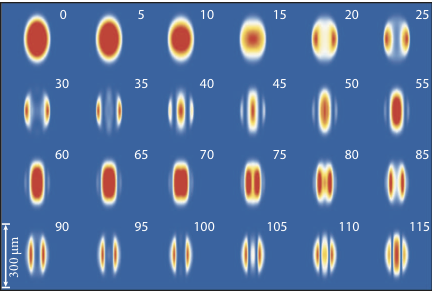
\includegraphics[width=2.5in]{evolution_reference.png}}
\qquad
\subfloat[Split-step simulation]{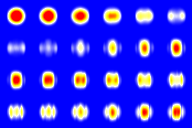
\includegraphics[width=2.5in]{evolution.png}}
\end{center}
\caption{Column density of the $\mid2\rangle$-component}
\label{evolution}
\end{figure}

\begin{figure}
\begin{center}
\subfloat[Without noise]{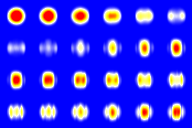
\includegraphics[width=2.5in]{evolution.png}}
\qquad
\subfloat[With noise, 4 ensembles]{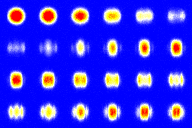
\includegraphics[width=2.5in]{evolution_noise.png}}
\end{center}
\caption{Column density of the $\mid2\rangle$-component}
\label{evolution-noise}
\end{figure}

First example of results obtained using the program is the rendering of density distribution of the $\mid2\rangle$-state. Namely, column density for one of the radial directions is rendered. Calculation parameters were taken from the paper "Spatially inhomogeneous phase evolution of a two-component Bose-Einstein condensate":
\[ N = 150000 \]
\[ a_{11} = 100.40 a_0, a_{12} = 97.66 a_0, a_{22} = 95.00 a_0 \]
\[ f_x = 11.962 \textrm{ Hz}, f_y = f_z = 97.62 \textrm{ Hz} \]
\[ m = 87 m_p \textrm{ (Rubidium)}\]
The result can be seen on Figure~\ref{evolution}. Evolution looks similar for both methods until 80 ms, then split-step method starts to produce significantly different picture. Introduction of quantum noise does not change the resulting picture much (at least, it is not noticeable for sparse lattices) - see Figure~\ref{evolution-noise}.

\begin{figure}
\begin{center}
\subfloat[Experimental results]{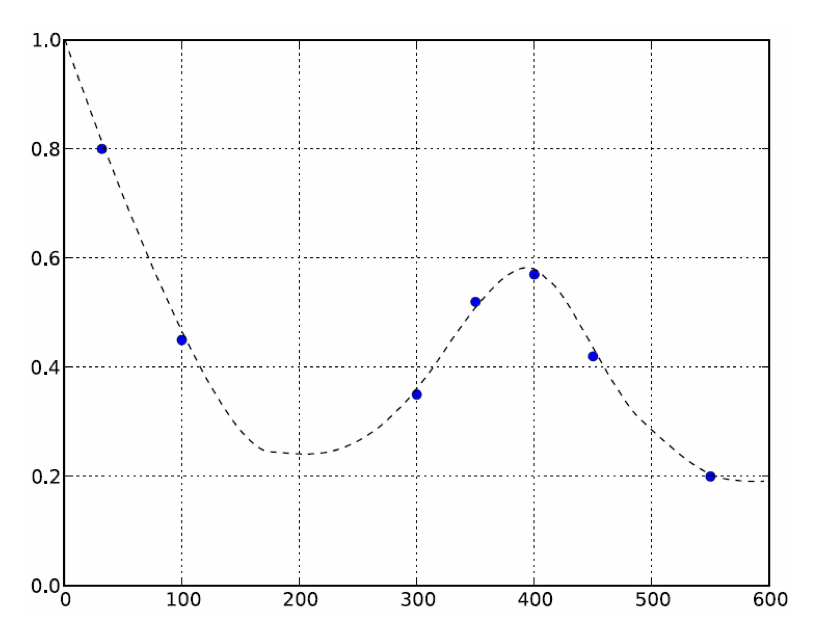
\includegraphics[width=4in]{visibility_reference.png}}\\
\subfloat[Split-step simulation]{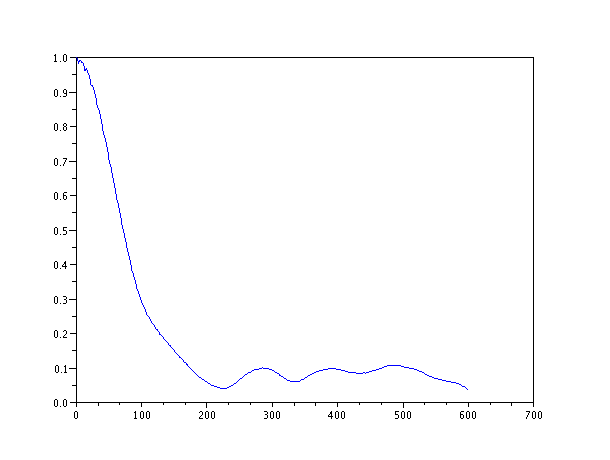
\includegraphics[width=4.5in]{visibility.png}}
\end{center}
\caption{Visibility over time graphs}
\label{visibility}
\end{figure}

Second example is the visibility graph, which shows quite unexpected behaviour too. The following parameters were used (taken from the presentation "Rephasing and Reversing the Nonlinear Dynamics of Two-Component Bose-Einstein Condensate", page 12:
\[ N = 70000 \]
\[ a_{11} = 100.44 a_0, a_{12} = 98.09 a_0, a_{22} = 95.47 a_0 \]
\[ f_x = 11 \textrm{ Hz}, f_y = f_z = 95 \textrm{ Hz} \]
\[ m = 87 m_p \textrm{ (Rubidium)}\]
For each time step, the vector of the system was rotated using matrix for angles from 0 to $2\pi$, with step 0.5, and the maximum of $\vert N_1 - N_2 \vert / (N_1 + N_2)$ was taken, producing the visibility. Resulting graph can be seen on Figure~\ref{visibility}. The results look somehow similar only in the beginning (during first 100 ms of evolution) and then the difference becomes apparent.

\end{document}
